\documentclass[12pt]{article}

\usepackage{graphicx}
\usepackage[margin=0.75in]{geometry}
\usepackage{multirow}

\usepackage{amsmath}
\usepackage{bm}
\newcommand{\m}[1]{\mathbf{\bm{#1}}}

\begin{document}

\section*{Homework 2 -- AMS 276}
\subsection*{Mickey Warner}
\bigskip
\bigskip

\section*{M1}

\noindent The likelihood for the proportionl hazards model with a Weibull as the baseline hazard function is given by:
\[ L(\m{y}|\m{x},\m{\nu},\alpha,\gamma,\beta) = \prod_{\{i:\nu_i=1\}} \alpha\gamma y_i^{\alpha-1} \times \prod_{i=1}^n\exp\left[-\gamma y_i^\alpha e^{x_i^\top\beta}\right] \]
\noindent I place independent gamma priors on $\alpha,\gamma$ and a normal prior on $\beta$:
\begin{eqnarray*}
\alpha &\sim& Gamma(1, 0.1) \\
\gamma &\sim& Gamma(1, 0.1) \\
\beta &\sim& Normal(0, 10^2)
\end{eqnarray*}
\noindent The full conditional for the joint parameter vector $(\alpha, \gamma, \beta)$ is proportional to the likelihood times each of the priors:
\[ \pi(\alpha,\gamma,\beta|\m{y},\m{x},\m{\nu}) = \prod_{\{i:\nu_i=1\}} \alpha\gamma y_i^{\alpha-1} \times \prod_{i=1}^n\exp\left[-\gamma y_i^\alpha e^{x_i^\top\beta}\right]\times e^{-0.1\alpha}e^{-0.1\gamma}\exp\left(-\frac{\beta^2}{2\cdot10^2}\right) \]
\noindent The parameters are updated jointly using Metropolis-Hastings updates. Their marginal posterior distributions and an estimate of the survival functions for the two groups (Aneuploid in blue and Diploid in red) are given at the end.

\section*{M2}

\noindent We define a partion $0=s_0 < s_1 < \cdots < s_J$ by the quantiles of the failure times. We let $J=20$, with $s_j$ being the $5\times j$th quantile.
\bigskip

\noindent The likelihood for the piece-wise constant hazard model is given by
\[ L(\m{y}|\m{x},\m{\nu},\m{\lambda},\m{\beta}) = \prod_{i=1}^n\prod_{j=1}^J(\lambda_j\exp^{\m{x}_i^\top\m{\beta}})^{\delta_{ij}\nu_i}\exp\left(-\delta_{ij}\left[\lambda_j(y_i-s_{j-1})+\sum_{g=1}^{j-1}\lambda_g(s_g-s_{g-1})\right]e^{\m{x}_i^\top\m{\beta}}\right) \]
\noindent This is the likelihood as given in ICS, which I noticed is different than the one you present on the slides. The difference is that you have the $\delta_{ij}$ term only over $\lambda_j$. I'm not sure what the consequences for this is, but I realized that it was necessary to include an intercept term, so $\m{\beta}=(\beta_0,\beta_1)$. For whatever reason, excluding the intercept made my estimates for $\beta_1$ off.
\bigskip

\noindent For priors, we have
\begin{eqnarray*}
\lambda_j &\overset{iid}\sim& Gamma(1, 1/10),~~~~~j=1,\ldots,J \\
\beta_j &\overset{iid}\sim& Normal(0, 10^2),~~~~~j=0,1 \\
\end{eqnarray*}
\noindent Again, I do a joint update of all the parameters. And yes, this is mostly so I don't have to derive individual full conditionals for each parameter.

\section*{M3}

\section*{Remarks about the figures}


\newpage
\subsection*{Figures for M1}
\begin{center}
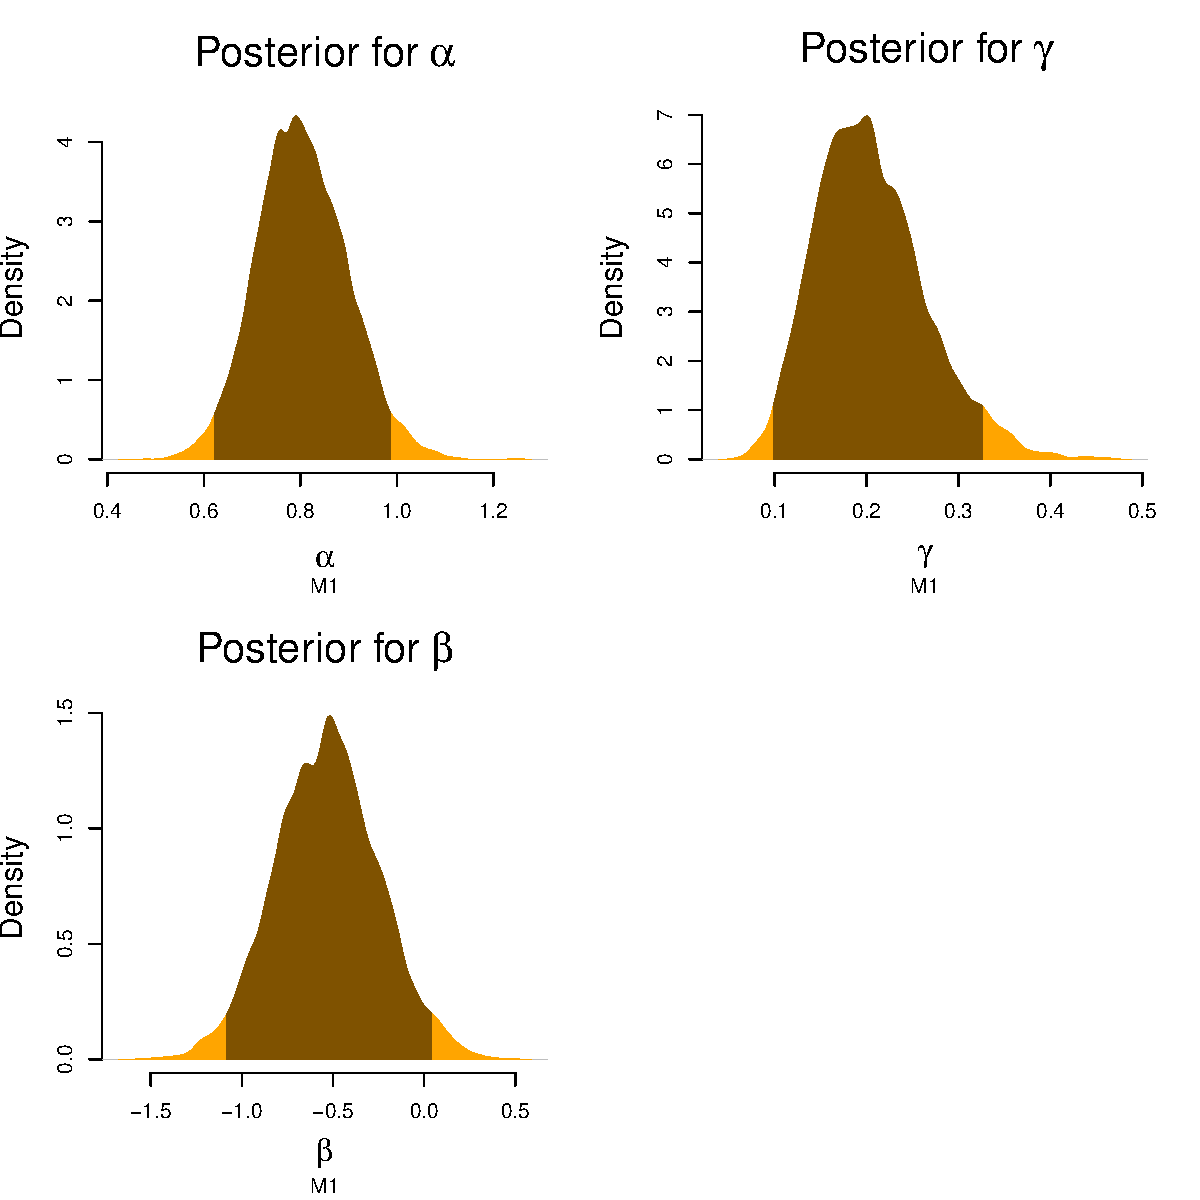
\includegraphics[scale=0.647]{figs/m1_post.pdf}
\bigskip
\bigskip

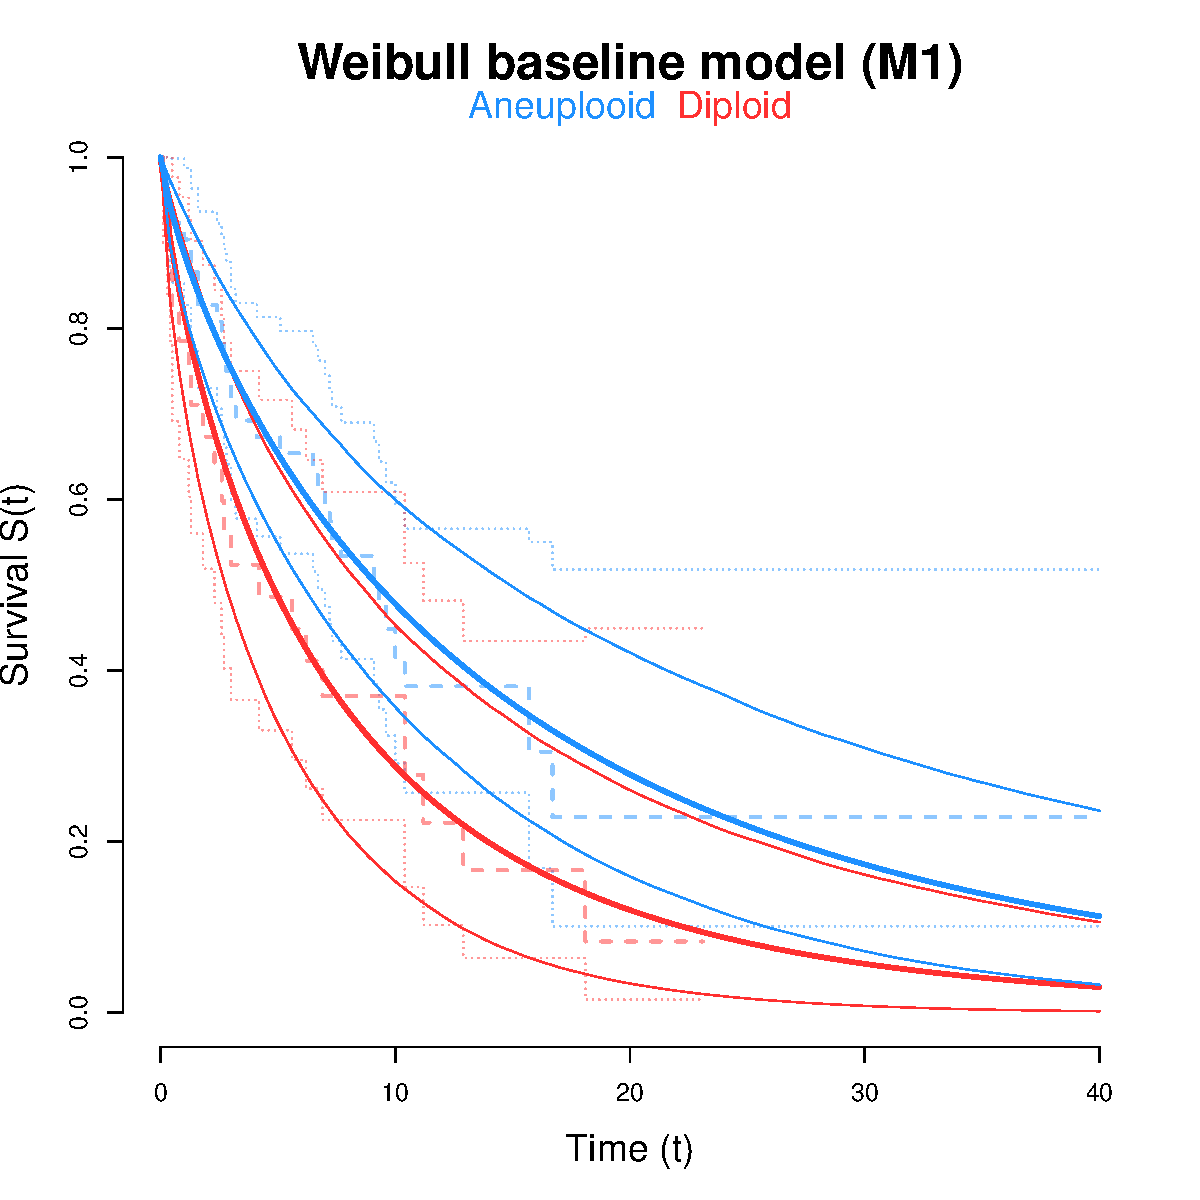
\includegraphics[scale=0.45]{figs/m1_surv.pdf}
\end{center}

\newpage
\subsection*{Figures for M2}
\begin{center}
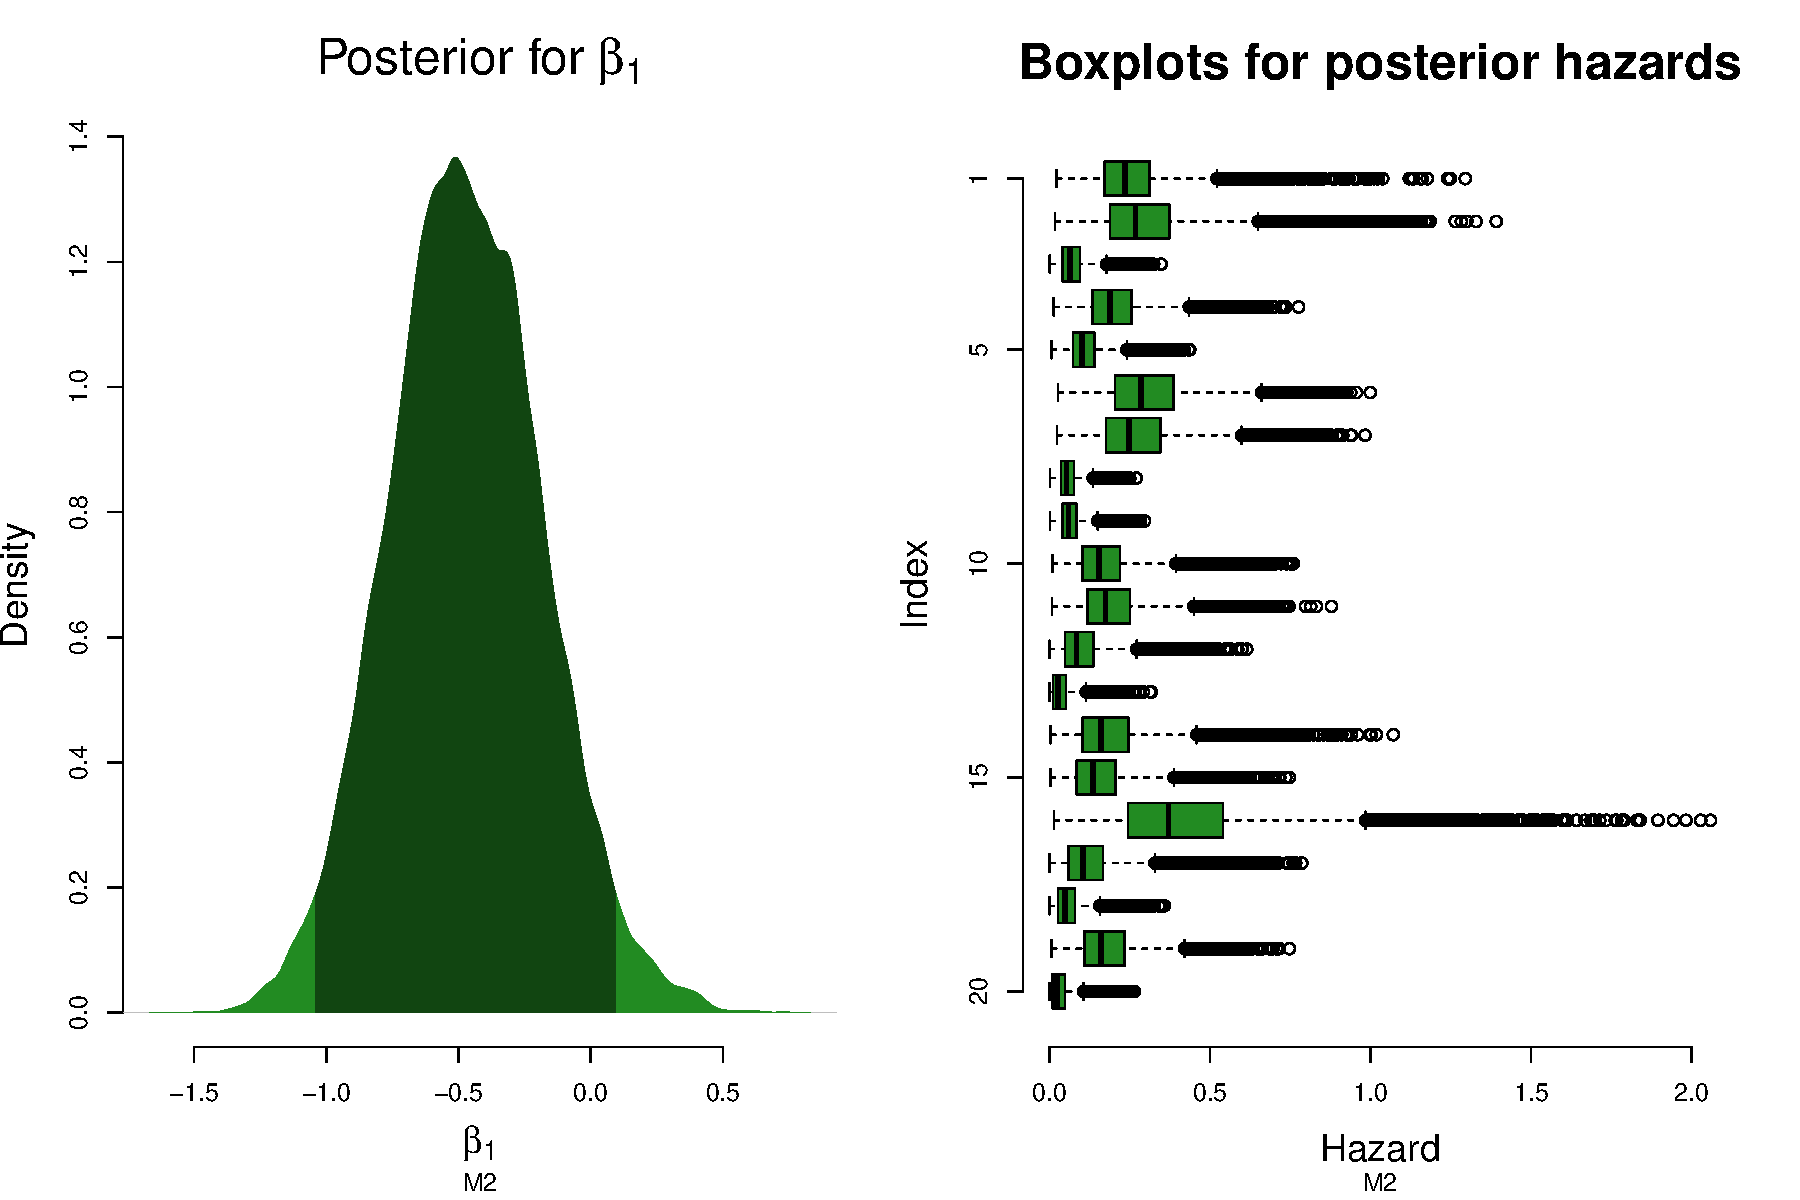
\includegraphics[scale=0.60]{figs/m2_post.pdf}
\bigskip
\bigskip

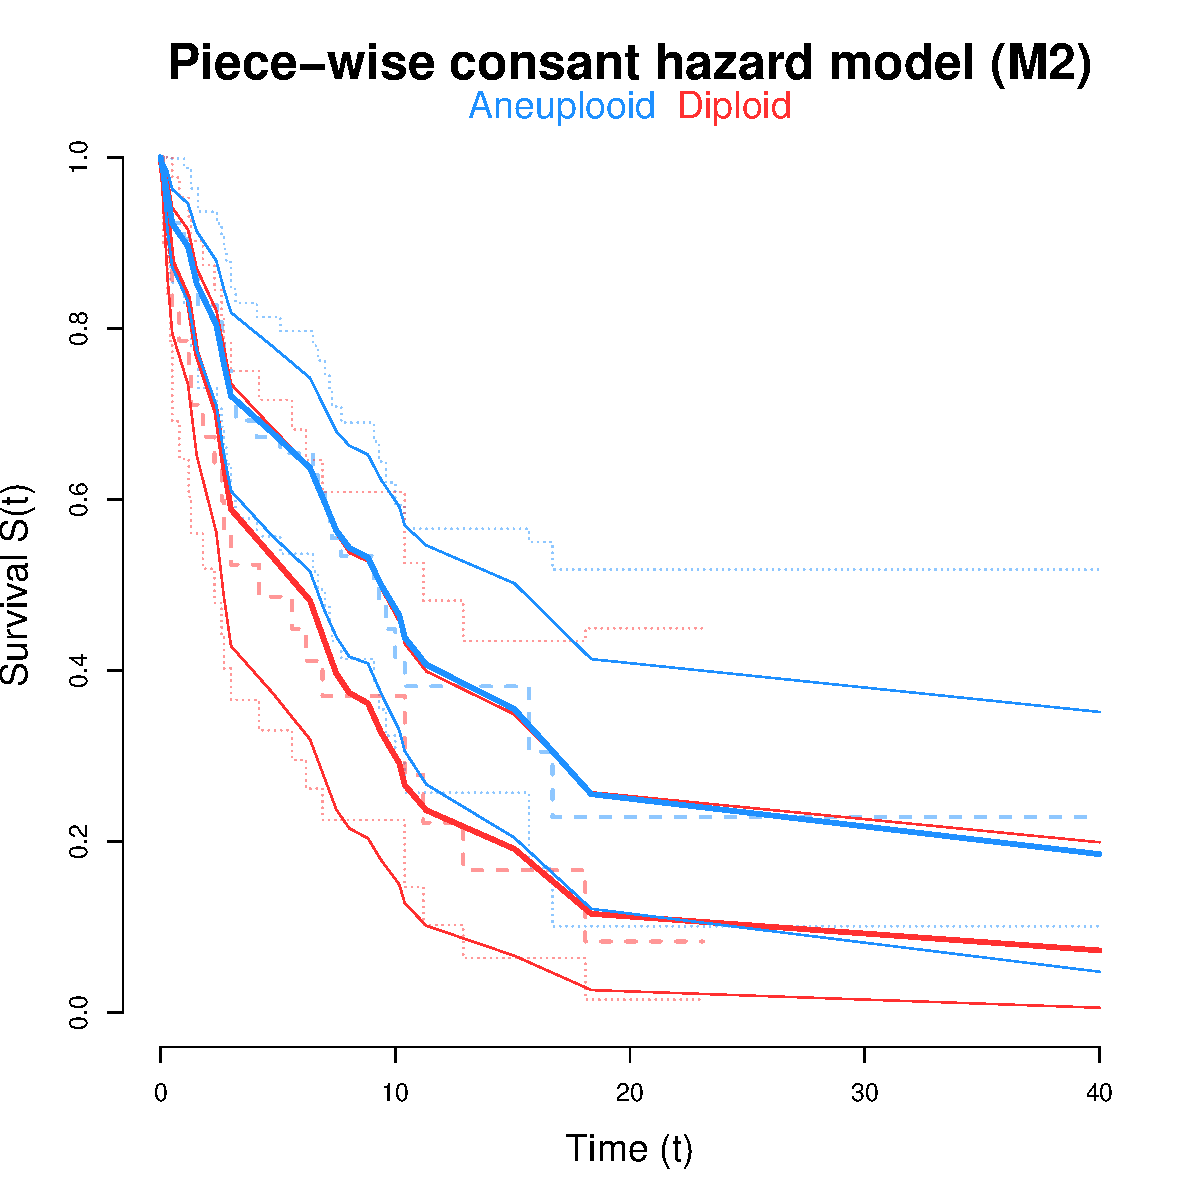
\includegraphics[scale=0.45]{figs/m2_surv.pdf}
\end{center}

\newpage
\subsection*{Figures for M3}
\begin{center}
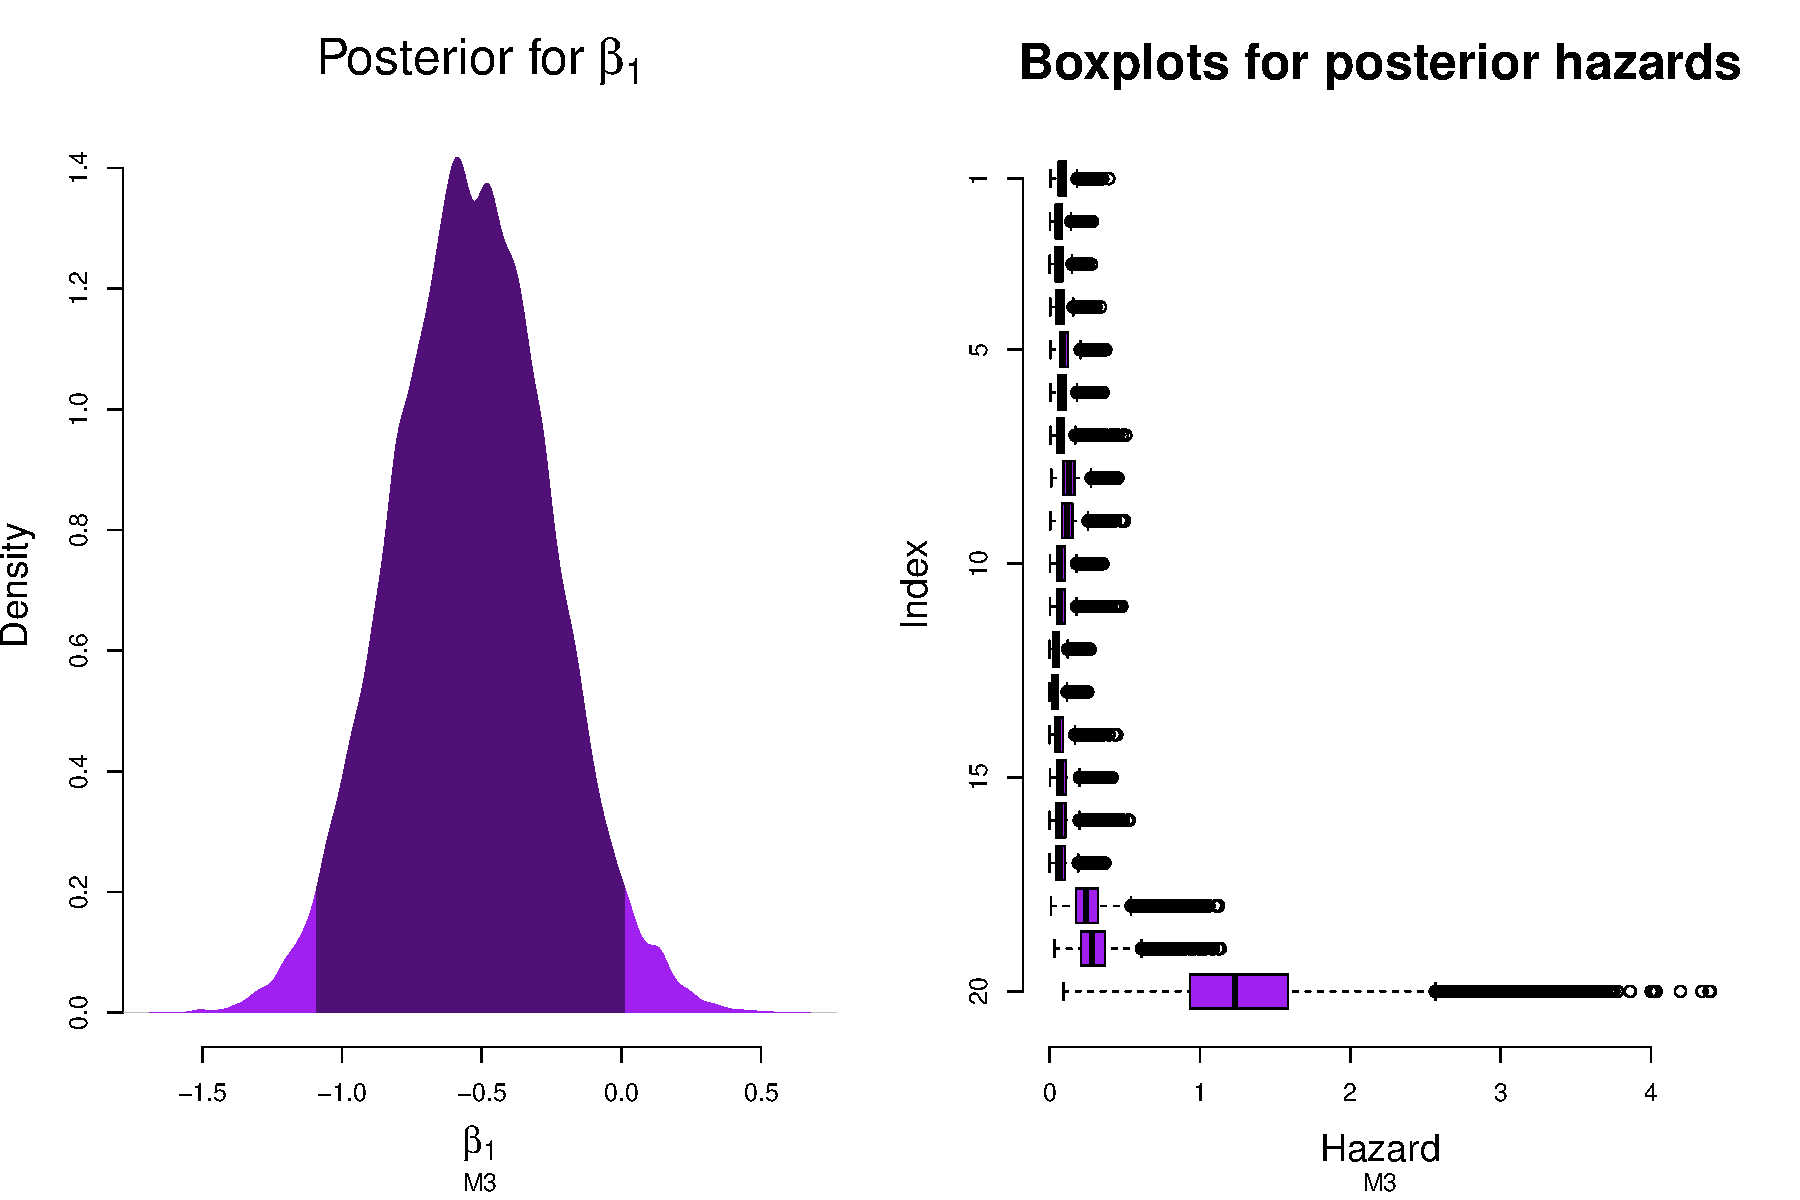
\includegraphics[scale=0.60]{figs/m3_post.pdf}
\bigskip
\bigskip

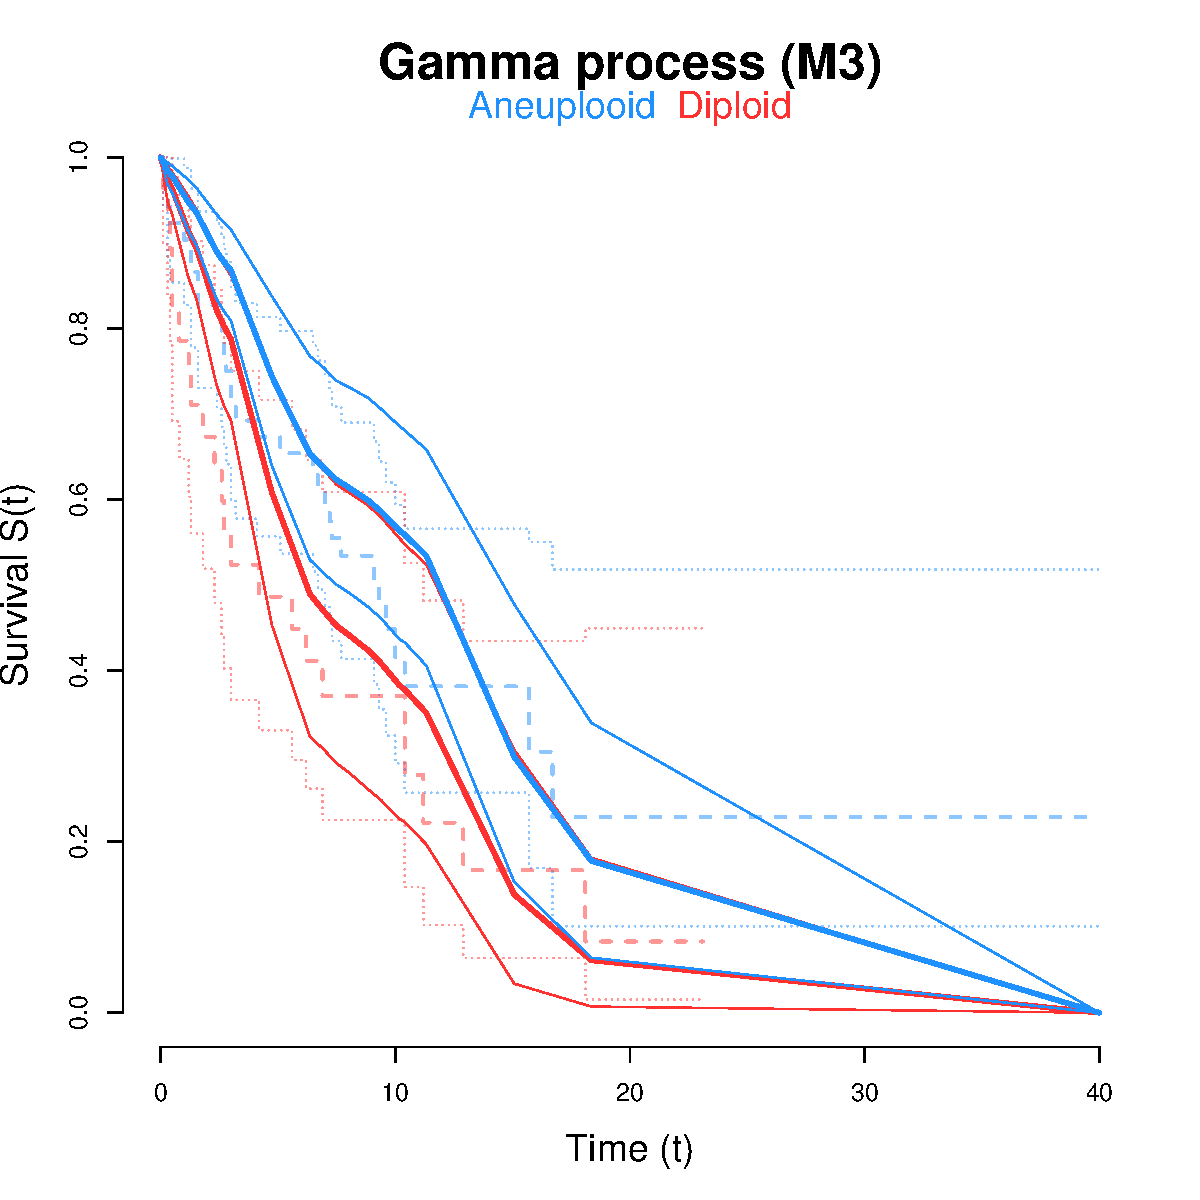
\includegraphics[scale=0.45]{figs/m3_surv.pdf}
\end{center}


\end{document}
